\begin{figure*}[!t]
\centering
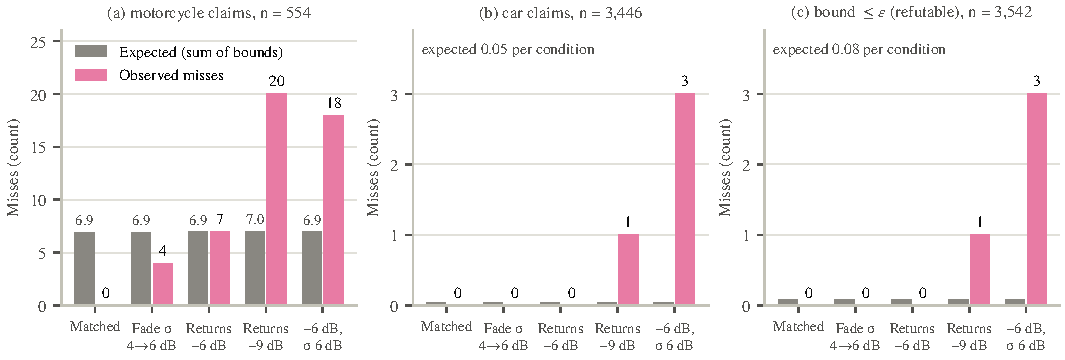
\includegraphics[width=\textwidth]{fig_calib.pdf}
\caption{Calibration of the miss bound against the ray-traced simulator (4,000 genuine claims per model condition; no traffic or faults; rain). Conditions: matched model; persistent-fade spread $\sigma_u$ raised from 4 to 6~dB; returns 6 or 9~dB weaker than modeled; returns 6~dB weaker with $\sigma_u = 6$~dB. Expected misses are the sum of the per-claim bounds, which the verifier computes under its nominal model in every condition; observed misses are claims for which every sample was free. (a) Motorcycle claims. (b) Car claims. (c) Claims whose bound is at most $\varepsilon$, i.e., the claims the formal tier would refute; all observed misses there were cars. Simulated data.}
\label{fig:calib}
\end{figure*}
